\chapter{\label{ch:polycubes2}Designing polycube assembly rules}

\minitoc

In the previous chapter, we used random input rules to explore properties of the corresponding distributions of output polycube shapes. However, the reverse problem is just as significant; given a target shape, how do you find a rule that assembles it?  

% Fully addressable is the easy solution.

A trivial solution would be to use \emph{fully addressable assembly}: simply assign a unique species to each cube and a unique colour to each pair of adjacent patches. This is similar to the design principle underlying DNA bricks (Section~\ref{sec:dna_tiles_bricks}), where every brick tile is unique. However, as was seen in Chapter~\ref{ch:polycubes1}, many shapes have alternative solutions requiring widely different numbers of unique components. See Figure~\ref{fig:addressable}, where a square tetromino is shown to have a variety of inputs assembling it, from the minimal solution with just a single species and one colour, up to the fully addressable solution with four species and four colours (\(\widetilde{K}_s = \widetilde{K}_c = 4\)). The intermediate solutions are not necessarily deterministic in terms of which position gets which species, but they will always assemble into the same shape.

% Andrew: Explain the significance of mismatched colours.

Meanwhile, the empty red region in Figure~\ref{fig:addressable}.b) shows combinations of \(\widetilde{K}_s\) and \(\widetilde{K}_c\) for which a solution is not possible. For example, if you use a single species, you cannot use more than one colour.

\begin{figure}[ht]
    \centering
    \begin{overpic}[width=\textwidth]{figures/solve/adressable.eps}
        \put(-10,480){a)}
        \put(360,580){b)}

        \put(370, 350){\makebox(0,0){\rotatebox{90}{Number of colours (\(\widetilde{K}_c\))}}}
        \put(600,-30){Number of species (\(\widetilde{K}_s\))}
    \end{overpic}
    \vspace{1em}
    %\includesvg[width=\textwidth, inkscapelatex=false]{figures/solve/adressable.svg}
    \caption{\(2 \times 2\) square polyomino assembled with different levels of complexity. \textbf{a)} Schematic of the input shape, consisting of four connected tiles. \textbf{b)} The green region shows possible assembly solutions, from the \emph{minimal solution} using a single species and a single colour (bottom left), to the \emph{fully addressable solution} using four species and colours (top right). The red region lacks solutions. }
    \label{fig:addressable}
\end{figure}

So, how do we find alternative and simpler input rules for a shape? Surely, there must exist a better method than sampling the space of all rules (as done in Chapter~\ref{ch:polycubes1})? This chapter presents an approach where \emph{satisfiability solving} is used to determine if a shape can be assembled from a given number of colours and species, thus automatically filling in solution landscapes such as the one shown in Figure~\ref{fig:addressable}. A complementary approach substituting similar species is also described in Section~\ref{sec:substitution_solving}.


\section{Satisfiability solving}

Building upon a published method for determining patchy particle interactions for unbounded structures \cite{romano2020designing}, it is possible to formulate and solve satisfiability problems that map onto assembly rules for the bounded polycube structures.

In essence, we formulate a boolean expression that, if true, means it is possible to assemble a given polycube topology using a given number of colours and species. We can then use a satisfiability solver to check if that expression is indeed solvable and, if it is, extract an assembly rule from the solution.

\subsection{Boolean expressions}

The boolean expression is written in conjunctive normal form (CNF), where variables are composed into clauses using \emph{NOT} (\(\lnot\)) and \emph{OR} (\(\lor\)) operators and where the clauses are joined by \emph{AND} (\(\land\)) operators. As a simple example, see the expression below:

\[
    (\lnot x_{rain} \lor x_{umbrella} \lor  \lnot x_{walk}) \land
    (\lnot x_{rainbow} \lor x_{rain}) \land
    (\lnot x_{rainbow} \lor x_{sunny})
\]

The first clause is \({true}\) for all values except when \(x_{rain}={true}\), \(x_{umbrella}={false}\) and \(x_{walk}=true\); so the solution of taking a walk in the rain without an umbrella is forbidden. This could also be written as an \emph{implication}: \(x_{rain} \land x_{walk} \implies x_{umbrella}\).

The following two clauses in the example above are the CNF form of another implication: \(x_{rainbow} \implies  x_{rain} \land x_{sunshine}\), stating that a rainbow implies that we have both rain and sunshine (we cannot have a rainbow without rain or without sunshine). The full expression is satisfiable, for example, if we set \(x_{sun}=true\), \(x_{rain}=false\), \(x_{walk}=false\), \(x_{umbrella}=false\), and \(x_{rainbow}=false\); ignoring the walk in the sunshine and remaining inside to work.

\subsection{Polycube formulation}

For the polycube problem, we introduce the following variables:
\begin{description}
    \item[\(x_{l,p,o}^{A}\)] (patch \(p\) at position \(l\) has orientation \(o\))
    \item[\(x_{c_i,c_j}^{B}\)] (colour \(c_i\) is compatible with colour \(c_j\))
    \item[\(x_{s,p,c}^{C}\)] (patch \(p\) on species \(s\) has colour \(c\))
    \item[\(x_{p_1,o_1,p_2,o_2}^{D}\)] (patch \(p_1\) with orientation \(o_1\) binds to patch \(p_2\) with orientation \(o_2\))
    \item[\(x_{l,p,c}^{F}\)] (patch \(p\) at position \(l\) has colour \(c\))
    \item[\(x_{s,p,o}^{O}\)] (patch \(p\) on species \(s\) has orientation \(o\))
    \item[\(x_{l,s,r}^{P}\)] (position \(l\) is occupied by species \(s\) rotated by \(r\))] 
\end{description}

We then formulate clauses to constrain the problem, seen in Table~\ref{tab:sat_clauses}. Clauses (i)-(vii) are the same as in \cite{romano2020designing} while the remaining are added, together with variables \(x^D\), \(x^A\) and \(x^O\) above, to include \emph{torsional restrictions}, meaning that patches need to bind at a compatible orientation (compared to being allowed to rotate freely).

\begin{table}[h!]
    \centering
    \begin{tabular}{|l|l|l|}
        \hline
        & Clause & Boolean expression \\ [0.5ex] 
        \hline
        \hline
        (i) & \(C^{B}_{c_i,c_j,c_k}\) & \(\neg x_{c_i,c_j}^{B} \lor \neg x_{c_i,c_k}^{B}\) \\ % Each colour is compatible with exactly one colour
        (ii) &  \(C^{C}_{s,p,c_k,c_l}\) & \(\neg x_{s, p, c_k}^{C} \lor \neg x_{s, p, c_l}^{C}\) \\ % Each patch is assigned exactly one colour
        (iii) & \(C^{P}_{l, s_i, r_i, s_j, r_j}\)  & \(\neg x_{l,s_i,r_i}^{P} \lor \neg x_{l,s_j,r_j}^{P} \) \\ % Each lattice position is occupied by a single species with one assigned rotation
        (iv) & \(C^{BF}_{l_i,p_i,c_i,l_j,p_j,c_j}\) & \(\left(x_{l_i,p_i,c_i}^{F} \land x_{l_j,p_j,c_j}^{F} \right) \Rightarrow x_{c_i,c_j}^{B}\) \\ % Colours of patches that interact in the target lattice must be compatible
        (v) & \(C^{rotC}_{l,s,r,p,c}\) & \(x_{l,s,r}^{P} \Rightarrow \left(x_{l,p,c}^{F} \Leftrightarrow x_{s, \phi_r(p), c}^{C}\right)\) \\ % The patches at a lattice position is set to have the patch colours of the rotated occupying species.
        (vi) & \(C^{all s}_{s}\)  & \(\bigvee_{\forall l, r} x_{l,s,r}^{P}\) \\ % All \widetilde{K}_s species are used for the lattice assembly
        (vii) & \(C^{all c}_{c}\)  & \(\bigvee_{\forall s, p} x_{s,p,c}^{C}\) \\ % All \widetilde{K}_c patch colours are used in the solution
        (iix) &  \(C^{O}_{s,p,o_k,o_l}\) & \(\neg x_{s, p, o_k}^{O} \lor \neg x_{s, p, o_l}^{O}\) \\ % Each patch is assigned exactly one orientation
        (ix) & \(C^{DA}_{l_i,p_i,c_i,l_j,p_j,c_j}\) & \(\left(x_{l_i,p_i,c_i}^{A} \land x_{l_j,p_j,c_j}^{A} \right) \Rightarrow x_{p_i,c_i,p_j,c_j}^{D}\) \\ % Orientation of patches that interact in the target lattice must be compatible
        (x) & \(C^{rotO}_{l,s,r,p,o}\) & \(x_{l,s,r}^{P} \Rightarrow \left(x_{l,p,o}^{A} \Leftrightarrow x_{s, \phi_r(p), o}^{O}\right)\) \\ % The patches at a lattice position is set to have the orientations of the rotated occupying species.
        \hline
    \end{tabular}
    \caption{SAT clauses. (i) Each colour is compatible with \textit{exactly one} colour. (ii) Each patch has \textit{exactly one} colour. (iii) Each lattice position contains a single species with an assigned rotation. (iv) Adjacent patches in the lattice must have compatible colours. (v) Patches at a lattice position are coloured according to the (rotated) occupying species. (vi) All \(\widetilde{K}_s\) species are required in the solution. (vii) All \(\widetilde{K}_c\) patch colours are required in the solution. (iix) Each patch is assigned \textit{exactly one} orientation. (ix) Adjacent patches in the target lattice must have the same orientation. (v)  Patches at a lattice position are oriented according to the (rotated) occupying species.}
    \label{tab:sat_clauses}

    % Andrew: I would make a full-page table with the English statement as an additional column.
    \end{table}

\subsection{On the importance of torsional interactions}

It would certainly be possible to use the solver without any constraints on the patch orientations (as it was done in \cite{romano2020designing}). However, if we wanted to use the stochastic assembler from Chapter~\ref{ch:polycubes1}, orientations would have to be assigned randomly, resulting in a combinatoric explosion of additional assembly paths.

More importantly, the assembly should benefit from torsional patch interaction (for 2D polyominoes, this corresponds to the requirement that tiles can be rotated in the plane but not flipped). Figure~\ref{fig:torsion} shows two versions of a simple rule, the only difference being the orientation of a single patch. While co-operative binding might, in such a case, benefit the desired square assembly, the self-limiting ability would be significantly improved if the patches were torsionally rigid.

\begin{figure}[ht]
    \centering
    \begin{overpic}[width=\textwidth]{figures/torsion.png}
        \put(0,470){a)}
        \put(550,500){b)}
    \end{overpic}
    \caption{The consequences of a rotated patch. \textbf{a)} A minimal solution (one species and one colour) for a \(2 \times 2\) square. \textbf{b)} The same rule as a), except one patch on is rotated by \(\frac{\pi}{2}\).}
    \label{fig:torsion}
\end{figure}


\subsection{Bounded structures}
Besides the torsional patches, another important difference to \cite{romano2020designing} is that the method presented here allows for bounded structures. This is achieved by adding species of type ``empty'' as a "shell" around the shape to ensure that empty patches remain unbound. Adding a clause \(x_{0,1}^{B}\) ensures that colour 0 (on the shell) always binds to 1 (on the boundary). 

We then add clauses \(x_{l,p,1}^{F}\) to constrain every boundary patch \(p\) at lattice position \(l\) to have the colour \(1\) and thereby not bind anything else. For example, in Figure~\ref{fig:sat_boundary}, where these boundary patches are seen coloured white (and bordering an empty square), we get the following 12 clauses:

\begin{equation}
    \begin{aligned}
        &x_{0,0,1}^{F} \land x_{0,1,1}^{F} \land x_{0,3,1}^{F} \land \\
        &x_{1,0,1}^{F} \land x_{1,2,1}^{F} \land x_{1,3,1}^{F} \land \\
        &x_{3,0,1}^{F} \land x_{3,1,1}^{F} \land x_{3,2,1}^{F} \land \\
        &x_{4,1,1}^{F} \land x_{4,2,1}^{F} \land x_{4,3,1}^{F}
    \end{aligned}
\end{equation}

Note that for 3D polycubes, there are six patches per species instead of the four seen in the 2D polyomino in Figure~\ref{fig:sat_boundary}. This also introduces 27 possible cube rotations, compared to the 4 square rotations defined for 2D.

The topology of the shape is enforced by clause (iv), \(\left(\lnot x_{l_1, p_1, c_1}^{F} \lor \lnot x_{l_2, p_2, c_2}^{F} \lor x_{c_1, c_2}^{B}\right)\) in CNF, making sure that if patch \(p_1\) on lattice position \(l_1\) binds to \(p_2\) on lattice position \(l_2\), their colours are compatible. Similarly, clause (ix) ensures that the patches have the same orientation.

% Figure of topology graph?

\begin{figure}[ht]
    \centering\includesvg[width=.5\textwidth, inkscapelatex=false]{figures/sat_boundary.svg}
    \caption{Bounded shape topology for satisfiability solving. Patches at the boundary of the shape (white) are constrained to only bind to ``empty''. 3D shapes are specified the same way, but with six patches per species.}
    \label{fig:sat_boundary}
\end{figure}

\subsection{Interaction matrix}
Compared to \cite{romano2020designing}, the interaction matrix is by default fixed. Thus, the \(x_{c_i,c_j}^{B}\) variable has fixed values and we only need to extract the values of \(x_{l,p,c}^{F}\) and \(x_{s,p,o}^{O}\) to construct the assembly rule. Note, however, that it is still possible to re-enable a variable interaction matrix, something which could prove useful for some shapes where, for example, self-complementary patches would result in a lower complexity.

Compared to the interaction matrix convention used in Chapter~\ref{ch:polycubes1}, where each colour \(c\) binds to \(-c\), the colour values in the SAT solver remain unsigned and instead pair each even colour \(c\) to the odd \(c+1\). The colour pairs are mapped back to the polycube convention when obtaining the solution.

\subsection{Assembly determinism}
Even if the SAT solver determines that a solution exists, it is still possible that the rule we get can also assemble into other shapes. Recall, once more, the ``giraffe duck'' shape from Figure~\ref{fig:UND}.b). If we solved for the shape with two neck cubes, the non-deterministic rule shown would be a perfectly valid solution according to the SAT solver, even though it can also produce giraffe ducks with any other neck length.

Because of this, we once again use the stochastic assembler to verify that the rule assembles into the correct shape every time. Each potential rule is evaluated a large number of times (by default \(100\)), calculating an assembly ratio. If the ratio is \(1\), the rule is considered bounded and deterministic and, as such, a valid solution.


\section{Finding the minimal assembly rule}

By iteratively ruling out lower values of \(\widetilde{K}_s\) and \(\widetilde{K}_c\), a minimal solution can be found, as detailed in Figure~\ref{fig:sat_alg}. It is also possible to generate and compare alternative solutions of varying complexity. While forbidding an undefined solution and retrying could in principle, continue until the computer runs out of memory (or the solution is disproven or valid), the results presented below used a limit of 100 retries before moving on.

The exploration of the solution landscape can also be done in parallel, with each combination of \(\widetilde{K}_s\) and \(\widetilde{K}_c\) explored concurrently.

\begin{figure}
    \centering
    \resizebox{\textwidth}{!}{% Graphic for TeX using PGF
% Title: /home/joakim/Documents/polycube/SAT_flow.dia
% Creator: Dia v0.97+git
% CreationDate: Thu May 27 10:43:08 2021
% For: joakim
% \usepackage{tikz}
% The following commands are not supported in PSTricks at present
% We define them conditionally, so when they are implemented,
% this pgf file will use them.
\ifx\du\undefined
  \newlength{\du}
\fi
\setlength{\du}{15\unitlength}
\begin{tikzpicture}[even odd rule]
\pgftransformxscale{1.000000}
\pgftransformyscale{-1.000000}
\definecolor{dialinecolor}{rgb}{0.000000, 0.000000, 0.000000}
\pgfsetstrokecolor{dialinecolor}
\pgfsetstrokeopacity{1.000000}
\definecolor{diafillcolor}{rgb}{1.000000, 1.000000, 1.000000}
\pgfsetfillcolor{diafillcolor}
\pgfsetfillopacity{1.000000}
\pgfsetlinewidth{0.100000\du}
\pgfsetdash{}{0pt}
\pgfsetmiterjoin
{\pgfsetcornersarced{\pgfpoint{0.000000\du}{0.000000\du}}\definecolor{diafillcolor}{rgb}{1.000000, 1.000000, 1.000000}
\pgfsetfillcolor{diafillcolor}
\pgfsetfillopacity{1.000000}
\fill (13.087793\du,24.536630\du)--(13.087793\du,26.436630\du)--(19.140293\du,26.436630\du)--(19.140293\du,24.536630\du)--cycle;
}{\pgfsetcornersarced{\pgfpoint{0.000000\du}{0.000000\du}}\definecolor{dialinecolor}{rgb}{0.000000, 0.000000, 0.000000}
\pgfsetstrokecolor{dialinecolor}
\pgfsetstrokeopacity{1.000000}
\draw (13.087793\du,24.536630\du)--(13.087793\du,26.436630\du)--(19.140293\du,26.436630\du)--(19.140293\du,24.536630\du)--cycle;
}% setfont left to latex
\definecolor{dialinecolor}{rgb}{0.000000, 0.000000, 0.000000}
\pgfsetstrokecolor{dialinecolor}
\pgfsetstrokeopacity{1.000000}
\definecolor{diafillcolor}{rgb}{0.000000, 0.000000, 0.000000}
\pgfsetfillcolor{diafillcolor}
\pgfsetfillopacity{1.000000}
\node[anchor=base,inner sep=0pt, outer sep=0pt,color=dialinecolor] at (16.114043\du,25.681630\du){Try \(N_c\) and \(N_t\)};
% setfont left to latex
\definecolor{dialinecolor}{rgb}{0.000000, 0.000000, 0.000000}
\pgfsetstrokecolor{dialinecolor}
\pgfsetstrokeopacity{1.000000}
\definecolor{diafillcolor}{rgb}{0.000000, 0.000000, 0.000000}
\pgfsetfillcolor{diafillcolor}
\pgfsetfillopacity{1.000000}
\node[anchor=base west,inner sep=0pt,outer sep=0pt,color=dialinecolor] at (27.290293\du,24.956775\du){Yes};
% setfont left to latex
\definecolor{dialinecolor}{rgb}{0.000000, 0.000000, 0.000000}
\pgfsetstrokecolor{dialinecolor}
\pgfsetstrokeopacity{1.000000}
\definecolor{diafillcolor}{rgb}{0.000000, 0.000000, 0.000000}
\pgfsetfillcolor{diafillcolor}
\pgfsetfillopacity{1.000000}
\node[anchor=base west,inner sep=0pt,outer sep=0pt,color=dialinecolor] at (24.240293\du,28.331775\du){No};
\pgfsetlinewidth{0.100000\du}
\pgfsetdash{}{0pt}
\pgfsetmiterjoin
{\pgfsetcornersarced{\pgfpoint{0.000000\du}{0.000000\du}}\definecolor{diafillcolor}{rgb}{1.000000, 1.000000, 1.000000}
\pgfsetfillcolor{diafillcolor}
\pgfsetfillopacity{1.000000}
\fill (39.101543\du,24.536630\du)--(39.101543\du,26.436630\du)--(42.064043\du,26.436630\du)--(42.064043\du,24.536630\du)--cycle;
}{\pgfsetcornersarced{\pgfpoint{0.000000\du}{0.000000\du}}\definecolor{dialinecolor}{rgb}{0.000000, 0.000000, 0.000000}
\pgfsetstrokecolor{dialinecolor}
\pgfsetstrokeopacity{1.000000}
\draw (39.101543\du,24.536630\du)--(39.101543\du,26.436630\du)--(42.064043\du,26.436630\du)--(42.064043\du,24.536630\du)--cycle;
}% setfont left to latex
\definecolor{dialinecolor}{rgb}{0.000000, 0.000000, 0.000000}
\pgfsetstrokecolor{dialinecolor}
\pgfsetstrokeopacity{1.000000}
\definecolor{diafillcolor}{rgb}{0.000000, 0.000000, 0.000000}
\pgfsetfillcolor{diafillcolor}
\pgfsetfillopacity{1.000000}
\node[anchor=base,inner sep=0pt, outer sep=0pt,color=dialinecolor] at (40.582793\du,25.681630\du){Done};
% setfont left to latex
\definecolor{dialinecolor}{rgb}{0.000000, 0.000000, 0.000000}
\pgfsetstrokecolor{dialinecolor}
\pgfsetstrokeopacity{1.000000}
\definecolor{diafillcolor}{rgb}{0.000000, 0.000000, 0.000000}
\pgfsetfillcolor{diafillcolor}
\pgfsetfillopacity{1.000000}
\node[anchor=base west,inner sep=0pt,outer sep=0pt,color=dialinecolor] at (37.640293\du,24.756775\du){Yes};
% setfont left to latex
\definecolor{dialinecolor}{rgb}{0.000000, 0.000000, 0.000000}
\pgfsetstrokecolor{dialinecolor}
\pgfsetstrokeopacity{1.000000}
\definecolor{diafillcolor}{rgb}{0.000000, 0.000000, 0.000000}
\pgfsetfillcolor{diafillcolor}
\pgfsetfillopacity{1.000000}
\node[anchor=base west,inner sep=0pt,outer sep=0pt,color=dialinecolor] at (33.890293\du,29.156775\du){No};
\pgfsetlinewidth{0.100000\du}
\pgfsetdash{}{0pt}
\pgfsetmiterjoin
\definecolor{diafillcolor}{rgb}{1.000000, 1.000000, 1.000000}
\pgfsetfillcolor{diafillcolor}
\pgfsetfillopacity{1.000000}
\fill (23.943082\du,23.300000\du)--(27.486164\du,25.486630\du)--(23.943082\du,27.673261\du)--(20.400000\du,25.486630\du)--cycle;
\definecolor{dialinecolor}{rgb}{0.000000, 0.000000, 0.000000}
\pgfsetstrokecolor{dialinecolor}
\pgfsetstrokeopacity{1.000000}
\draw (23.943082\du,23.300000\du)--(27.486164\du,25.486630\du)--(23.943082\du,27.673261\du)--(20.400000\du,25.486630\du)--cycle;
% setfont left to latex
\definecolor{dialinecolor}{rgb}{0.000000, 0.000000, 0.000000}
\pgfsetstrokecolor{dialinecolor}
\pgfsetstrokeopacity{1.000000}
\definecolor{diafillcolor}{rgb}{0.000000, 0.000000, 0.000000}
\pgfsetfillcolor{diafillcolor}
\pgfsetfillopacity{1.000000}
\node[anchor=base,inner sep=0pt, outer sep=0pt,color=dialinecolor] at (23.943082\du,25.681630\du){Satisfiable?};
\pgfsetlinewidth{0.100000\du}
\pgfsetdash{}{0pt}
\pgfsetmiterjoin
\definecolor{diafillcolor}{rgb}{1.000000, 1.000000, 1.000000}
\pgfsetfillcolor{diafillcolor}
\pgfsetfillopacity{1.000000}
\fill (33.444978\du,22.430375\du)--(37.941584\du,25.486630\du)--(33.444978\du,28.542886\du)--(28.948372\du,25.486630\du)--cycle;
\definecolor{dialinecolor}{rgb}{0.000000, 0.000000, 0.000000}
\pgfsetstrokecolor{dialinecolor}
\pgfsetstrokeopacity{1.000000}
\draw (33.444978\du,22.430375\du)--(37.941584\du,25.486630\du)--(33.444978\du,28.542886\du)--(28.948372\du,25.486630\du)--cycle;
% setfont left to latex
\definecolor{dialinecolor}{rgb}{0.000000, 0.000000, 0.000000}
\pgfsetstrokecolor{dialinecolor}
\pgfsetstrokeopacity{1.000000}
\definecolor{diafillcolor}{rgb}{0.000000, 0.000000, 0.000000}
\pgfsetfillcolor{diafillcolor}
\pgfsetfillopacity{1.000000}
\node[anchor=base,inner sep=0pt, outer sep=0pt,color=dialinecolor] at (33.444978\du,25.281630\du){Bounded \&};
% setfont left to latex
\definecolor{dialinecolor}{rgb}{0.000000, 0.000000, 0.000000}
\pgfsetstrokecolor{dialinecolor}
\pgfsetstrokeopacity{1.000000}
\definecolor{diafillcolor}{rgb}{0.000000, 0.000000, 0.000000}
\pgfsetfillcolor{diafillcolor}
\pgfsetfillopacity{1.000000}
\node[anchor=base,inner sep=0pt, outer sep=0pt,color=dialinecolor] at (33.444978\du,26.081630\du){Deterministic?};
\pgfsetlinewidth{0.100000\du}
\pgfsetdash{}{0pt}
\pgfsetmiterjoin
{\pgfsetcornersarced{\pgfpoint{0.000000\du}{0.000000\du}}\definecolor{diafillcolor}{rgb}{1.000000, 1.000000, 1.000000}
\pgfsetfillcolor{diafillcolor}
\pgfsetfillopacity{1.000000}
\fill (30.669978\du,29.741575\du)--(30.669978\du,32.441575\du)--(36.272478\du,32.441575\du)--(36.272478\du,29.741575\du)--cycle;
}{\pgfsetcornersarced{\pgfpoint{0.000000\du}{0.000000\du}}\definecolor{dialinecolor}{rgb}{0.000000, 0.000000, 0.000000}
\pgfsetstrokecolor{dialinecolor}
\pgfsetstrokeopacity{1.000000}
\draw (30.669978\du,29.741575\du)--(30.669978\du,32.441575\du)--(36.272478\du,32.441575\du)--(36.272478\du,29.741575\du)--cycle;
}% setfont left to latex
\definecolor{dialinecolor}{rgb}{0.000000, 0.000000, 0.000000}
\pgfsetstrokecolor{dialinecolor}
\pgfsetstrokeopacity{1.000000}
\definecolor{diafillcolor}{rgb}{0.000000, 0.000000, 0.000000}
\pgfsetfillcolor{diafillcolor}
\pgfsetfillopacity{1.000000}
\node[anchor=base,inner sep=0pt, outer sep=0pt,color=dialinecolor] at (33.471228\du,30.886575\du){Forbid current};
% setfont left to latex
\definecolor{dialinecolor}{rgb}{0.000000, 0.000000, 0.000000}
\pgfsetstrokecolor{dialinecolor}
\pgfsetstrokeopacity{1.000000}
\definecolor{diafillcolor}{rgb}{0.000000, 0.000000, 0.000000}
\pgfsetfillcolor{diafillcolor}
\pgfsetfillopacity{1.000000}
\node[anchor=base,inner sep=0pt, outer sep=0pt,color=dialinecolor] at (33.471228\du,31.686575\du){solution};
\pgfsetlinewidth{0.100000\du}
\pgfsetdash{}{0pt}
\pgfsetbuttcap
{
\definecolor{diafillcolor}{rgb}{0.000000, 0.000000, 0.000000}
\pgfsetfillcolor{diafillcolor}
\pgfsetfillopacity{1.000000}
% was here!!!
\pgfsetarrowsend{stealth}
\definecolor{dialinecolor}{rgb}{0.000000, 0.000000, 0.000000}
\pgfsetstrokecolor{dialinecolor}
\pgfsetstrokeopacity{1.000000}
\draw (19.188296\du,25.486630\du)--(20.400000\du,25.486630\du);
}
\pgfsetlinewidth{0.100000\du}
\pgfsetdash{}{0pt}
\pgfsetbuttcap
{
\definecolor{diafillcolor}{rgb}{0.000000, 0.000000, 0.000000}
\pgfsetfillcolor{diafillcolor}
\pgfsetfillopacity{1.000000}
% was here!!!
\pgfsetarrowsend{stealth}
\definecolor{dialinecolor}{rgb}{0.000000, 0.000000, 0.000000}
\pgfsetstrokecolor{dialinecolor}
\pgfsetstrokeopacity{1.000000}
\draw (27.486164\du,25.486630\du)--(28.948372\du,25.486630\du);
}
\pgfsetlinewidth{0.100000\du}
\pgfsetdash{}{0pt}
\pgfsetbuttcap
{
\definecolor{diafillcolor}{rgb}{0.000000, 0.000000, 0.000000}
\pgfsetfillcolor{diafillcolor}
\pgfsetfillopacity{1.000000}
% was here!!!
\pgfsetarrowsend{stealth}
\definecolor{dialinecolor}{rgb}{0.000000, 0.000000, 0.000000}
\pgfsetstrokecolor{dialinecolor}
\pgfsetstrokeopacity{1.000000}
\draw (37.941584\du,25.486630\du)--(39.101543\du,25.486630\du);
}
\pgfsetlinewidth{0.100000\du}
\pgfsetdash{}{0pt}
\pgfsetbuttcap
{
\definecolor{diafillcolor}{rgb}{0.000000, 0.000000, 0.000000}
\pgfsetfillcolor{diafillcolor}
\pgfsetfillopacity{1.000000}
% was here!!!
\pgfsetarrowsend{stealth}
\definecolor{dialinecolor}{rgb}{0.000000, 0.000000, 0.000000}
\pgfsetstrokecolor{dialinecolor}
\pgfsetstrokeopacity{1.000000}
\draw (33.444978\du,28.542886\du)--(33.471228\du,29.741575\du);
}
\pgfsetlinewidth{0.100000\du}
\pgfsetdash{}{0pt}
\pgfsetmiterjoin
\pgfsetbuttcap
{
\definecolor{diafillcolor}{rgb}{0.000000, 0.000000, 0.000000}
\pgfsetfillcolor{diafillcolor}
\pgfsetfillopacity{1.000000}
% was here!!!
\pgfsetarrowsend{stealth}
{\pgfsetcornersarced{\pgfpoint{0.000000\du}{0.000000\du}}\definecolor{dialinecolor}{rgb}{0.000000, 0.000000, 0.000000}
\pgfsetstrokecolor{dialinecolor}
\pgfsetstrokeopacity{1.000000}
\draw (23.943082\du,27.673261\du)--(23.943082\du,28.932418\du)--(20.986832\du,28.932418\du)--(20.986832\du,30.191575\du);
}}
\pgfsetlinewidth{0.100000\du}
\pgfsetdash{}{0pt}
\pgfsetmiterjoin
\pgfsetbuttcap
{
\definecolor{diafillcolor}{rgb}{0.000000, 0.000000, 0.000000}
\pgfsetfillcolor{diafillcolor}
\pgfsetfillopacity{1.000000}
% was here!!!
\pgfsetarrowsend{stealth}
{\pgfsetcornersarced{\pgfpoint{0.000000\du}{0.000000\du}}\definecolor{dialinecolor}{rgb}{0.000000, 0.000000, 0.000000}
\pgfsetstrokecolor{dialinecolor}
\pgfsetstrokeopacity{1.000000}
\draw (23.943082\du,27.673261\du)--(23.943082\du,28.932418\du)--(26.950582\du,28.932418\du)--(26.950582\du,30.191575\du);
}}
\pgfsetlinewidth{0.100000\du}
\pgfsetdash{}{0pt}
\pgfsetmiterjoin
{\pgfsetcornersarced{\pgfpoint{0.000000\du}{0.000000\du}}\definecolor{diafillcolor}{rgb}{1.000000, 1.000000, 1.000000}
\pgfsetfillcolor{diafillcolor}
\pgfsetfillopacity{1.000000}
\fill (13.140293\du,21.036775\du)--(13.140293\du,23.736775\du)--(19.090293\du,23.736775\du)--(19.090293\du,21.036775\du)--cycle;
}{\pgfsetcornersarced{\pgfpoint{0.000000\du}{0.000000\du}}\definecolor{dialinecolor}{rgb}{0.000000, 0.000000, 0.000000}
\pgfsetstrokecolor{dialinecolor}
\pgfsetstrokeopacity{1.000000}
\draw (13.140293\du,21.036775\du)--(13.140293\du,23.736775\du)--(19.090293\du,23.736775\du)--(19.090293\du,21.036775\du)--cycle;
}% setfont left to latex
\definecolor{dialinecolor}{rgb}{0.000000, 0.000000, 0.000000}
\pgfsetstrokecolor{dialinecolor}
\pgfsetstrokeopacity{1.000000}
\definecolor{diafillcolor}{rgb}{0.000000, 0.000000, 0.000000}
\pgfsetfillcolor{diafillcolor}
\pgfsetfillopacity{1.000000}
\node[anchor=base,inner sep=0pt, outer sep=0pt,color=dialinecolor] at (16.115293\du,22.181775\du){Start};
% setfont left to latex
\definecolor{dialinecolor}{rgb}{0.000000, 0.000000, 0.000000}
\pgfsetstrokecolor{dialinecolor}
\pgfsetstrokeopacity{1.000000}
\definecolor{diafillcolor}{rgb}{0.000000, 0.000000, 0.000000}
\pgfsetfillcolor{diafillcolor}
\pgfsetfillopacity{1.000000}
\node[anchor=base,inner sep=0pt, outer sep=0pt,color=dialinecolor] at (16.115293\du,22.981775\du){\(N_c = N_t = 0\)};
\pgfsetlinewidth{0.100000\du}
\pgfsetdash{}{0pt}
\pgfsetbuttcap
{
\definecolor{diafillcolor}{rgb}{0.000000, 0.000000, 0.000000}
\pgfsetfillcolor{diafillcolor}
\pgfsetfillopacity{1.000000}
% was here!!!
\pgfsetarrowsend{stealth}
\definecolor{dialinecolor}{rgb}{0.000000, 0.000000, 0.000000}
\pgfsetstrokecolor{dialinecolor}
\pgfsetstrokeopacity{1.000000}
\draw (16.114729\du,23.786099\du)--(16.114446\du,24.486897\du);
}
\pgfsetlinewidth{0.100000\du}
\pgfsetdash{}{0pt}
\pgfsetmiterjoin
{\pgfsetcornersarced{\pgfpoint{0.000000\du}{0.000000\du}}\definecolor{diafillcolor}{rgb}{1.000000, 1.000000, 1.000000}
\pgfsetfillcolor{diafillcolor}
\pgfsetfillopacity{1.000000}
\fill (18.404332\du,30.191575\du)--(18.404332\du,32.441575\du)--(23.569332\du,32.441575\du)--(23.569332\du,30.191575\du)--cycle;
}{\pgfsetcornersarced{\pgfpoint{0.000000\du}{0.000000\du}}\definecolor{dialinecolor}{rgb}{0.000000, 0.000000, 0.000000}
\pgfsetstrokecolor{dialinecolor}
\pgfsetstrokeopacity{1.000000}
\draw (18.404332\du,30.191575\du)--(18.404332\du,32.441575\du)--(23.569332\du,32.441575\du)--(23.569332\du,30.191575\du)--cycle;
}% setfont left to latex
\definecolor{dialinecolor}{rgb}{0.000000, 0.000000, 0.000000}
\pgfsetstrokecolor{dialinecolor}
\pgfsetstrokeopacity{1.000000}
\definecolor{diafillcolor}{rgb}{0.000000, 0.000000, 0.000000}
\pgfsetfillcolor{diafillcolor}
\pgfsetfillopacity{1.000000}
\node[anchor=base,inner sep=0pt, outer sep=0pt,color=dialinecolor] at (20.986832\du,31.511575\du){Increase \(N_c\)};
\pgfsetlinewidth{0.100000\du}
\pgfsetdash{}{0pt}
\pgfsetmiterjoin
{\pgfsetcornersarced{\pgfpoint{0.000000\du}{0.000000\du}}\definecolor{diafillcolor}{rgb}{1.000000, 1.000000, 1.000000}
\pgfsetfillcolor{diafillcolor}
\pgfsetfillopacity{1.000000}
\fill (24.419332\du,30.191575\du)--(24.419332\du,32.441575\du)--(29.481832\du,32.441575\du)--(29.481832\du,30.191575\du)--cycle;
}{\pgfsetcornersarced{\pgfpoint{0.000000\du}{0.000000\du}}\definecolor{dialinecolor}{rgb}{0.000000, 0.000000, 0.000000}
\pgfsetstrokecolor{dialinecolor}
\pgfsetstrokeopacity{1.000000}
\draw (24.419332\du,30.191575\du)--(24.419332\du,32.441575\du)--(29.481832\du,32.441575\du)--(29.481832\du,30.191575\du)--cycle;
}% setfont left to latex
\definecolor{dialinecolor}{rgb}{0.000000, 0.000000, 0.000000}
\pgfsetstrokecolor{dialinecolor}
\pgfsetstrokeopacity{1.000000}
\definecolor{diafillcolor}{rgb}{0.000000, 0.000000, 0.000000}
\pgfsetfillcolor{diafillcolor}
\pgfsetfillopacity{1.000000}
\node[anchor=base,inner sep=0pt, outer sep=0pt,color=dialinecolor] at (26.950582\du,31.511575\du){Increase \(N_t\)};
\pgfsetlinewidth{0.100000\du}
\pgfsetdash{}{0pt}
\pgfsetmiterjoin
\pgfsetbuttcap
{
\definecolor{diafillcolor}{rgb}{0.000000, 0.000000, 0.000000}
\pgfsetfillcolor{diafillcolor}
\pgfsetfillopacity{1.000000}
% was here!!!
\pgfsetarrowsend{stealth}
{\pgfsetcornersarced{\pgfpoint{0.000000\du}{0.000000\du}}\definecolor{dialinecolor}{rgb}{0.000000, 0.000000, 0.000000}
\pgfsetstrokecolor{dialinecolor}
\pgfsetstrokeopacity{1.000000}
\draw (20.986832\du,32.491191\du)--(20.986832\du,33.000000\du)--(12.347500\du,33.000000\du)--(12.347500\du,25.486630\du)--(13.087793\du,25.486630\du);
}}
\pgfsetlinewidth{0.100000\du}
\pgfsetdash{}{0pt}
\pgfsetmiterjoin
\pgfsetbuttcap
{
\definecolor{diafillcolor}{rgb}{0.000000, 0.000000, 0.000000}
\pgfsetfillcolor{diafillcolor}
\pgfsetfillopacity{1.000000}
% was here!!!
\pgfsetarrowsend{stealth}
{\pgfsetcornersarced{\pgfpoint{0.000000\du}{0.000000\du}}\definecolor{dialinecolor}{rgb}{0.000000, 0.000000, 0.000000}
\pgfsetstrokecolor{dialinecolor}
\pgfsetstrokeopacity{1.000000}
\draw (26.950582\du,32.441575\du)--(26.950582\du,33.000000\du)--(12.347500\du,33.000000\du)--(12.347500\du,25.486630\du)--(13.087793\du,25.486630\du);
}}
\pgfsetlinewidth{0.100000\du}
\pgfsetdash{}{0pt}
\pgfsetmiterjoin
\pgfsetbuttcap
{
\definecolor{diafillcolor}{rgb}{0.000000, 0.000000, 0.000000}
\pgfsetfillcolor{diafillcolor}
\pgfsetfillopacity{1.000000}
% was here!!!
\pgfsetarrowsend{stealth}
{\pgfsetcornersarced{\pgfpoint{0.000000\du}{0.000000\du}}\definecolor{dialinecolor}{rgb}{0.000000, 0.000000, 0.000000}
\pgfsetstrokecolor{dialinecolor}
\pgfsetstrokeopacity{1.000000}
\draw (33.471228\du,32.441575\du)--(33.471228\du,33.000000\du)--(12.347500\du,33.000000\du)--(12.347500\du,25.486630\du)--(13.087793\du,25.486630\du);
}}
\end{tikzpicture}
}
    \caption{Algorithm for finding the minimal solution using SAT. Even if a solution is found to be satisfiable it might not assemble correctly every time. Additional solutions for a given \(\widetilde{K}_c\) and \(\widetilde{K}_s\) are found by explicitly forbidding the current solution. Alternatively, it is possible to use a solver like relsat to obtain multiple solutions. }
    \label{fig:sat_alg}
\end{figure}

\section{Simplification by substitution}
\label{sec:substitution_solving}
An alternative and complementary approach is to substitute species that are similar, removing duplicates. Starting from a fully addressable solution, any pair of species \(s_1\) and \(s_2\) with the same configuration of patches are tested. If we can remove \(s_1\) and replace the patches complementary to it with ones complementary to the patches of \(s_2\) and still get the correct output shape, we have successfully simplified the rule. This substitution continues until all species pairs have been tried.

\section{Example solves}
\label{sec:example_solves}
This section presents a set of different shapes solved to demonstrate the SAT solver method described above.

\paragraph{Swan} A more sophisticated version of the ``giraffe duck'' from Figure~\ref{fig:UND}, the Swan shape has a fixed neck length of one intermediate cube, as shown in Figure~\ref{fig:swan}.a). Figure~\ref{fig:swan}.b) shows the solution landscape, where valid deterministic solutions can be found along the upper diagonal. Many of the configurations classified as undefined (UND) because they are not fully deterministic, still assemble at a high ratio. This indicates that these \(\widetilde{K}_s\), \(\widetilde{K}_c\) combinations still could provide useful solutions.

\begin{figure}[ht]
    \centering
    %\includesvg[width=0.6\textwidth, inkscapelatex=false]{figures/solve/swan.svg}
    \begin{overpic}[width=\textwidth]{figures/solve/swan.eps}
        \put(10,450){a)}
        \put(360,450){b)}

        \put(380, 260){\makebox(0,0){\rotatebox{90}{Number of colours (\(\widetilde{K}_c\))}}}
        \put(490, 0){Number of species (\(\widetilde{K}_s\))}
    \end{overpic}
    \caption{Finding assembly rules for a polycube ``Swan''. \textbf{a)} Visualisation of the swan shape. \textbf{b)} Solution landscape.}
    \label{fig:swan}
\end{figure}

\paragraph{Polyomino J} With the 2D option enabled, the solver requires fewer clauses as it only needs to check four patches and four rotations per particle. Here this is used to explore the solution landscape for a polyomino shaped like a letter \textbf{J}, shown in Figure~\ref{fig:letter_J}.a). Figure~\ref{fig:letter_J}.b) shows the resulting solution landscape, where the minimal solution is just one species less than the fully addressable one. This can be explained by the lack of symmetry and modularity in the shape, where only the species used for the ``endpoints'' can be reused. 

\begin{figure}[ht]
    \centering
    %\includesvg[width=0.6\textwidth, inkscapelatex=false]{figures/solve/letter_J.svg}
    \begin{overpic}[width=\textwidth]{figures/solve/letter_J.eps}
        \put(10,480){a)}
        \put(300,480){b)}

        \put(300, 260){\makebox(0,0){\rotatebox{90}{Number of colours (\(\widetilde{K}_c\))}}}
        \put(460, 0){Number of species (\(\widetilde{K}_s\))}
    \end{overpic}
    \caption{Finding assembly rules for a polyomino ``letter J''. \textbf{a)} Visualisation of the shape. \textbf{b)} Solution landscape.}
    \label{fig:letter_J}
\end{figure}

\paragraph{Robot} The ``robot'' shape seen in Figure~\ref{fig:robot}.a) consists of more cubes than the previous examples, thereby resulting in the larger assembly landscape seen in Figure~\ref{fig:robot}.b). Once again, the valid solutions clearly follow the border region between the blue UND region of solutions with varying assembly ratio and the red region where no solution is possible.

\begin{figure}[ht]
    \centering
    %\includesvg[width=0.8\textwidth, inkscapelatex=true]{figures/solve/robot.svg}
    \begin{overpic}[width=\textwidth]{figures/solve/robot.eps}
        \put(10,480){a)}
        \put(360,480){b)}

        \put(380, 260){\makebox(0,0){\rotatebox{90}{Number of colours (\(\widetilde{K}_c\))}}}
        \put(530, -10){Number of species (\(\widetilde{K}_s\))}
    \end{overpic}
    \caption{Finding assembly rules for a polycube ``robot''. \textbf{a)} Visualisation of the robot shape. \textbf{b)} Solution landscape.}
    \label{fig:robot}
\end{figure}

\paragraph{Hollow cube} The hollow \(3 \times 3 \times 3\) cube (Figure~\ref{fig:hollow_cube}.a) is a good example of a larger structure (20 cubes) that still has a very low complexity solution, as seen in Figure~\ref{fig:hollow_cube},b). This low complexity can be explained by the high symmetry of the shape, needing just a single species for the vertices and another species for the edges.

\begin{figure}[ht]
    \centering
    %\includesvg[width=\textwidth, inkscapelatex=false]{figures/solve/cube.svg}
    \begin{overpic}[width=\textwidth]{figures/solve/cube.eps}
        \put(10,480){a)}
        \put(320,600){b)}

        \put(350, 310){\makebox(0,0){\rotatebox{90}{Number of colours (\(\widetilde{K}_c\))}}}
        \put(520, -10){Number of species (\(\widetilde{K}_s\))}
    \end{overpic}
    \caption{Finding assembly rules for a hollow \(3 \times 3 \times 3\) cube. \textbf{a)} Visualisation of the \(3 \times 3 \times 3\) cube shape. \textbf{b)} Solution landscape.}
    \label{fig:hollow_cube}
\end{figure}

\paragraph{Solid cube} Figure~\ref{fig:solid_cube} shows the solution landscape for a solid \(3 \times 3 \times 3\) cube. While it is visible also for the hollow cube, the sharp border of valid solutions along the diagonal seen in previous solutions is now less clear. This could be due to an increasing number of alternative solutions available for a given \(\widetilde{K}_s\), \(\widetilde{K}_c\) position, leading to some positions getting classified as UND while a valid solution could be found through further retries.

\begin{figure}[ht]
    \centering
    %\includesvg[width=\textwidth, inkscapelatex=false]{figures/solve/filled_cube.svg}
    \begin{overpic}[width=\textwidth]{figures/solve/filled_cube.eps}
        \put(10,480){a)}
        \put(300,600){b)}

        \put(300, 320){\makebox(0,0){\rotatebox{90}{Number of colours (\(\widetilde{K}_c\))}}}
        \put(510, -10){Number of species (\(\widetilde{K}_s\))}
    \end{overpic}
    \caption{Finding assembly rules for a solid \(3 \times 3 \times 3\) cube. \textbf{a)} Visualisation of the \(3 \times 3 \times 3\) cube shape. \textbf{b)} Solution landscape.}
    \label{fig:solid_cube}
\end{figure}

\section{Scalability analysis}

% Ard: I can think of lots of questions, such as -- how does this method scale? When does it break down? For the systems like the 16mers in chapter 3, how does it compare with what you find by random sampling of rules etc...
% Discuss scaling and when it breaks down. How does it scale with size of the system. Plot number of clauses needed on the grid


\section{Comparison to random sampling results}

% Ard: Compare ch4 back to previous results. Make grids from random samples, colour by frequency.

% 1) Take a high probability structure (e.g. the cube) and see how often different rules are found by random sampling  --- is it roughly ture that P(ruleset) ~ 2^(size)  -- log P(ruleset) ~ size of ruleset 
% 2) I would do this for some of the say 16mers or other 2D structures e.g. in the paper with Iain -- we simply found the K by looking at the shortest code found by sampling. Question" how good is this in practice. --  you did this as well in your plots.


\section{Assembly in a continuous model}
While the stochastic assembler works well to test determinism, a more realistic assembly can be achieved through patchy particle simulation.

\subsection{Patchy particle simulation}
\label{sec:patchy_particles}

% Andrew: Describe! Diffusion, in position and orientation. Hence need to constrain interactions tightly to ensure good mapping to more abstract models.

Besides discrete tile models, self-assembly can also be modelled using Molecular Dynamics simulations of rigid-body spheres called \emph{patchy particles}. Each particle has a number of patches that bind when they come in contact with another complementary patch.

One such patchy particle simulator is included as part of the oxDNA package \cite{rovigatti2015comparison}. It was, for example, used by Romano et al., as seen in Figure~\ref{fig:patchy_particles}, to verify the patchy interactions designed by their SAT-solver method \cite{romano2020designing}. The same patchy particle model is used here. However, to account for the polycube requirement of patch orientation alignment, the model has been modified to include torsional interactions.


\begin{figure}[ht]
  \centering
  \begin{overpic}[width=\textwidth]{figures/patchy_particles.png}
    \put(0,310){a)}
    \put(280,310){b)}
    \put(650,310){c)}
  \end{overpic}
  \caption{Patchy particle simulation, adapted from \cite{romano2020designing}. \textbf{a)} The unit cell of a tetrastack lattice build with patchy particles. \textbf{b)} Simulation snapshot of a forming tetrastack lattice. Note the free-flowing particles that have not yet attached the growing latttice they surround. \textbf{c)} Tetrastack particle energy plotted over simulation time for different temperatures. Sudden drops in energy correspond to nucleation events (where the lattices start forming).}
  \label{fig:patchy_particles}
\end{figure}


\begin{eqnarray*}
 \mathbf{p}_1 &=& R \left( 0,1,0\right)\\
 \mathbf{p}_2 &=& R \left( 0,-1,0 \right)  \\
 \mathbf{p}_3 &=& R \left( 0,0,1 \right)\\
 \mathbf{p}_4 &=& R \left(  0, 0, -1 \right)  \\
 \mathbf{p}_5 &=& R \left( 1,0,0 \right)\\
 \mathbf{p}_6 &=& R \left( -1, 0, 0 \right)  ,
\end{eqnarray*}

\begin{equation}
V_{\rm patch}(\mathbf{r}_{ij},\mathbf{\Omega}_{ij}) = \delta_{ab} V_{\rm pdist}(r_p) V_{\rm angle}(\theta_a, \theta_b, \theta_3), 
\end{equation}

\begin{eqnarray*}
\cos \theta_a &=&  \mathbf{\hat{r}}_{ij} \cdot \mathbf{\hat{p}}_a \\
\cos \theta_b &=&  \mathbf{-\hat{r}}_{ij} \cdot \mathbf{\hat{p}}_b \\
\cos \theta_3 &=&  \mathbf{o}_{a} \cdot \mathbf{o}_b  \\
\end{eqnarray*}

\begin{equation}
    V_{\rm angle}(\theta_a, \theta_b, \theta_3) = V_{\rm agmod}(\theta_a) V_{\rm agmod}(\theta_b)
    V_{\rm agmod}(\theta_3) ,
\end{equation}

\begin{equation}
V_{\rm angmod}(\theta) = \begin{cases}
	V_{\rm mod}(\theta, a, \theta^0)  & \text{if $ \theta^0 - \Delta < \theta < \theta^0 + \Delta  $},\\
	V_{\rm smooth} (\theta, b, \theta^0 - \Delta^c) & \text{if $\theta^0 - \Delta^c < \theta < \theta^0-\Delta $},\\
	V_{\rm smooth} (\theta, b, \theta^0 + \Delta^c) & \text{if $\theta^0 + \Delta < \theta < \theta^0+\Delta^c$},\\
	0 & \text{otherwise}.
	\end{cases} 
\end{equation}

\begin{equation}
\label{eq:smooth}
V_{\rm smooth} (x, b, x^c) = b(x^c - x)^2, 
\end{equation}
and
\begin{equation}
V_{\rm mod} (\theta, a, \theta^0) = 1 - a (\theta-\theta^0)^2.
\end{equation}

\begin{equation}
    \label{eq_patch}
    V_{\rm pdist}(r_p) =  \begin{cases} 
                          %-1.001 \delta_{ij} e^{- \left( \frac{r_p}{\alpha} \right)^{10}} - C & \text{if $r_p \leq r_{\rm pmax}  $}\\
                          -1.001  \exp{\left[- \left( \frac{r_p}{\alpha} \right)^{10}\right]} - C & \text{if $r_p \leq r_{\rm pmax}  $} \\
                          0 & \text{otherwise}
                        \end{cases}
    %e^{ -\left( \frac{r - \delta}{\sigma} \right)^2} 
\end{equation}

\begin{equation}
    f_{\rm exc}(r,\epsilon,\sigma,r^{\star}) = \begin{cases}
	V_{\rm LJ}(r, \epsilon, \sigma) & \text{if $r < r^{\star} $},\\
	\epsilon V_{\rm smooth} (r, b, r^c) & \text{if $r^{\star} < r < r^c$},\\
	0 & \text{otherwise}.
	\end{cases} 
\end{equation}

\begin{equation} 
V_{\rm LJ}(r,  \sigma) = 8 \left[ \left(\frac{\sigma}{r}\right) ^{12} - \left(\frac{\sigma}{r}\right) ^{6} \right].
\end{equation}
%that is truncated using a quadratic smoothening function from Eq. \eqref{eq:smooth}.

\subsection{Yield calculation}
The patchy particle simulation yields are calculated using edge-induced subgraph isomorphism. 

We annotate \(\sigma(G,H) == \text{True}\) if the graph \(G\) is an edge-induced subgraph of the graph \(G\), meaning that

The connectivity graph \(G_i\) for each assembled particle cluster is compared to the graph for the intended shape \(G_{correct}\). If \(G_i\) is a large enough edge-induced subgraph of \(G_{correct}\), it contributes to the yield with its fraction of correctly assembled particles:
\begin{equation}
    Y_{c} = \sum_{G_i \in c} \begin{cases} 
           \frac{\left|N(G_i)\right|}{\left|N(G_{correct})\right|} & \text{if}  \\
                          0 & \text{otherwise}
                        \end{cases}
\end{equation}

\subsection{Preliminary simulation results}
Since there are different \emph{narrow types} available, corresponding to slightly different patch interaction potential widths, we start by simulating the structure stability for each potential and for a range of different temperatures. As seen in Figure~\ref{fig:narrow_types}, higher temperatures and lower narrow types cause the assembly to fall apart and the potential energy to increase. For narrow type 0, there is still some connectivity for the higher temperatures, with the energy oscillating as particles bind and unbind, but for higher narrow types, the oscillations grow less, and the particles remain unbound.

\begin{figure}[ht]
    \centering
    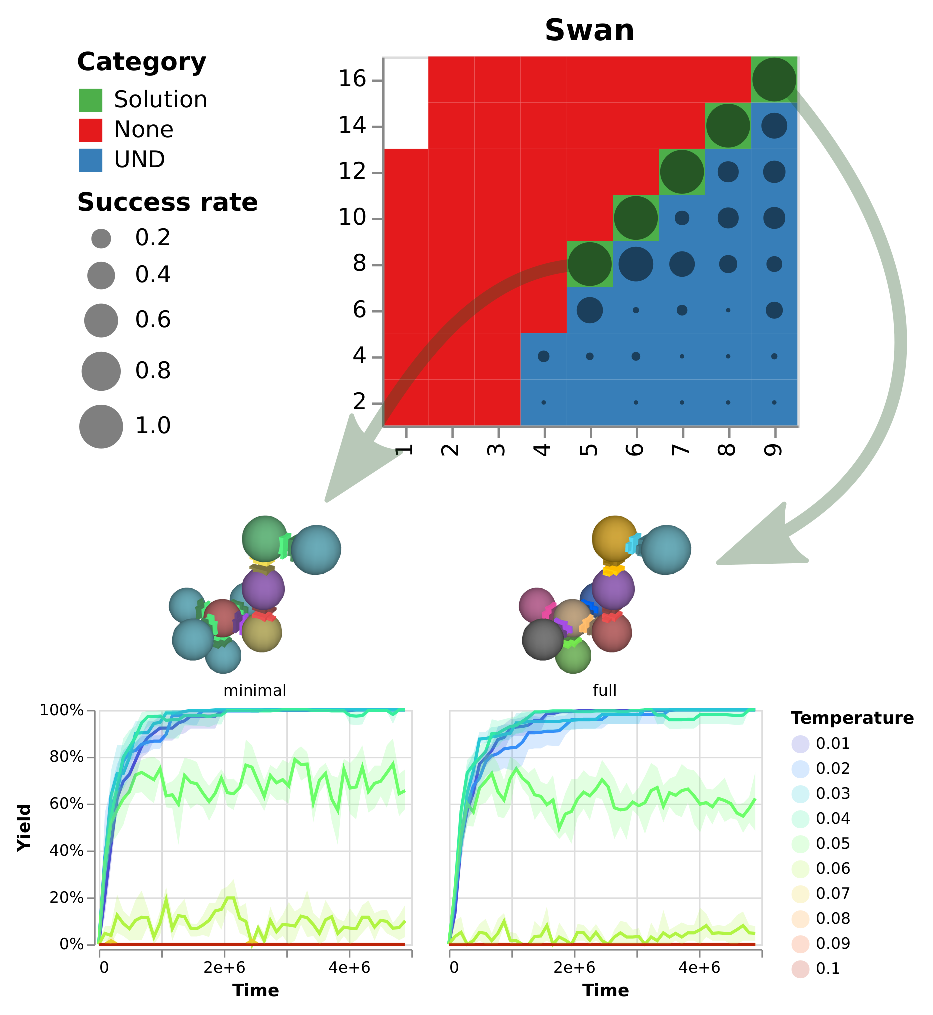
\includegraphics[width=\linewidth]{figures/patchysim/swanKinetics.eps}
    \caption{Assembly kinetics for different designs of the ``Swan'' shape. The left column shows the  \href{https://akodiat.github.io/polycubes/?assemblyMode=stochastic&rule=89010204000099099e00a20c0101861000000115920000009501020000000119020000000101021c0000010102000020010102008e00}{fully addressable solution} while the right is the \href{https://akodiat.github.io/polycubes/?assemblyMode=stochastic&rule=8f0b080b000b0b00000012008791000000000c0005000000000088000000}{minimal solution} found. Solid lines are mean values from 5 duplicate simulations, error bands show the 95\% confidence interval band. Each simulation is done using the narrow type \(0\) potential (patch width = \(2.346\)) at a \(0.1\) particle density. Temperature and time is measured in simulation units.}
    \label{fig:swanKinetics}
\end{figure}

\begin{figure*}[ht]
    \centering
    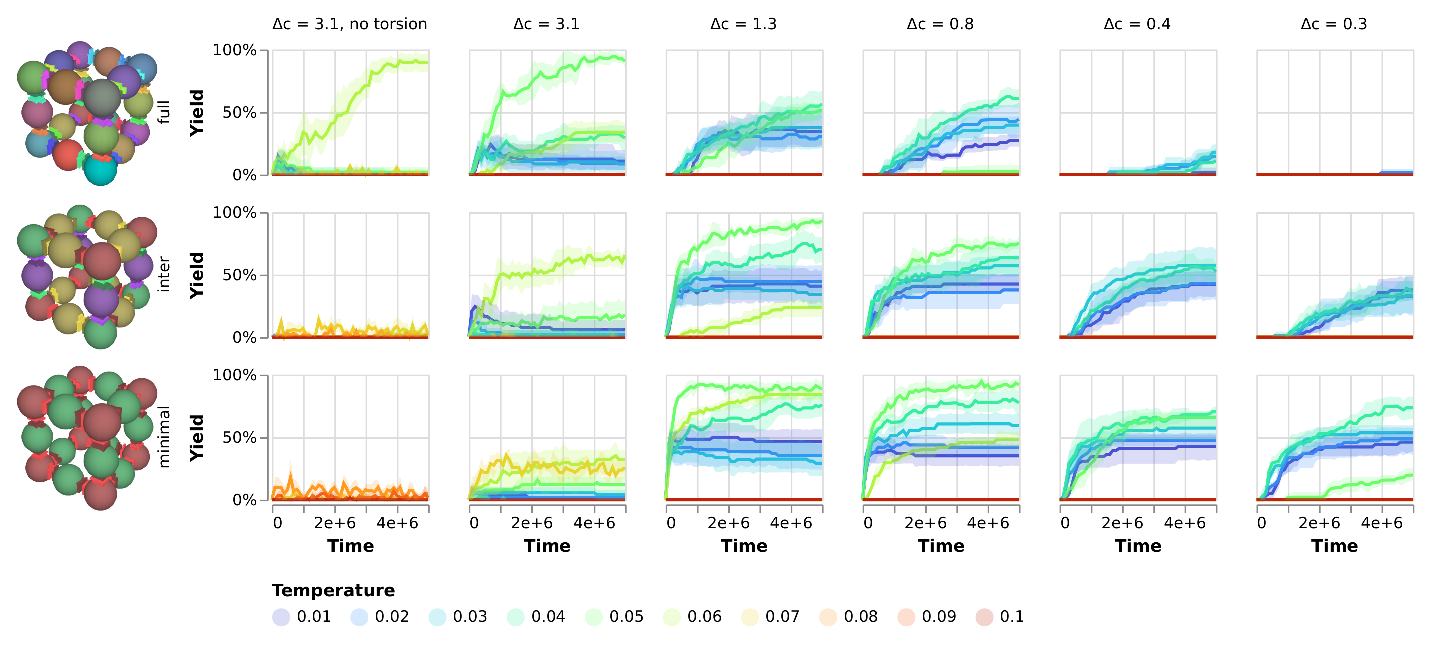
\includegraphics[width=\linewidth]{figures/patchysim/cubePotentials.eps}
    \caption{Assembly yield for hollow \(3 \times 3 \times 3\) cube designs. The top row shows the \href{https://akodiat.github.io/polycubes/?assemblyMode=stochastic&rule=00040109020c000089110200001491010218000001018e1c002001259e000000a5290200002ca901b200000001019a30963401010200863801010200ba00013d02400000bd450200b600c5010248ae4c01010200ce00e101d20000000101ca5000000101c254de000159d600a25c010102000000d9610200}{fully addressable solution}, using 20 species and 24 colours. The middle row shows an \href{https://akodiat.github.io/polycubes/?assemblyMode=stochastic&rule=90000800000600040090000d000000008b8d000011860000}{intermediate solution}, using 4 species and 4 colours. The bottom row shows the \href{https://akodiat.github.io/polycubes/?assemblyMode=stochastic&rule=070000070500868700000000}{minimal solution}, using 2 species and 1 colour. Columns correspond to different interaction potentials, with the leftmost column showing wide patches without torsion. The remaining columns show torsional patches with decreasing patch width. Solid lines are mean values from 5 duplicate simulations, and error bands show the 95\% confidence interval band. Each simulation has a \(0.1\) particle density.}
    \label{fig:cubePotentials}
\end{figure*}

\begin{figure*}[ht]
    \centering
    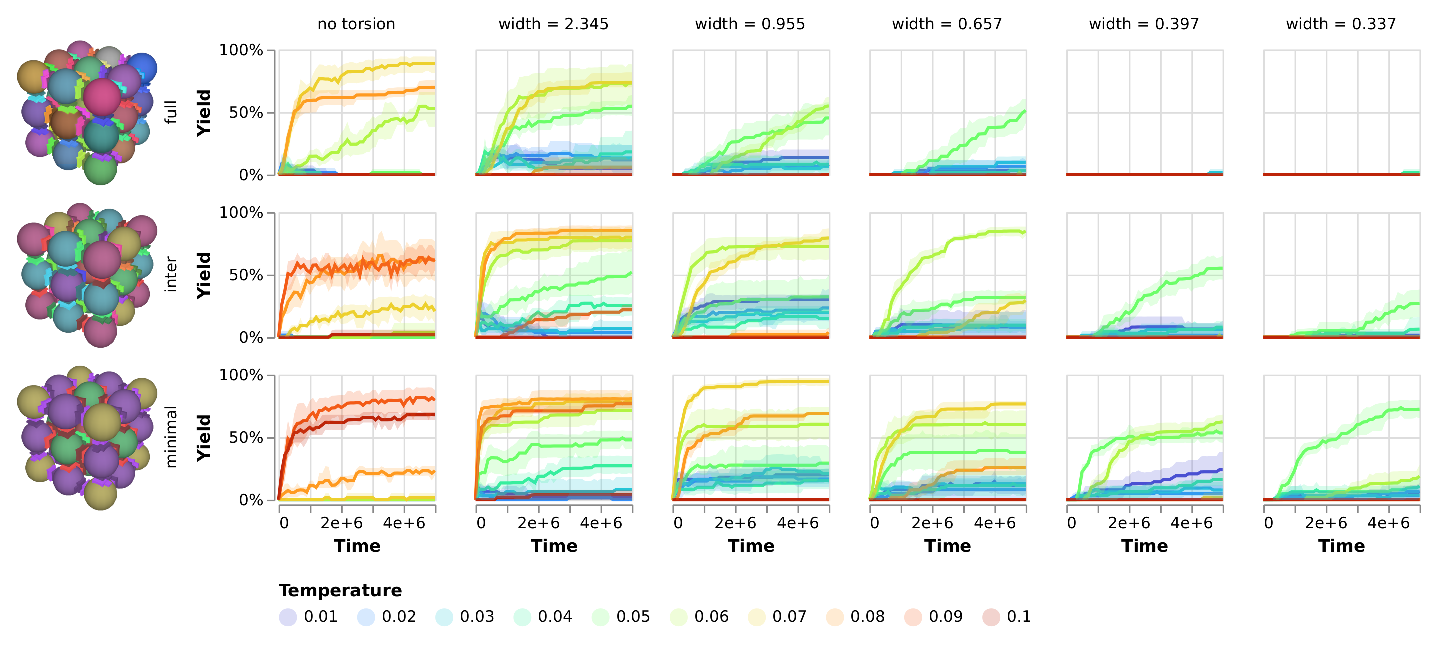
\includegraphics[width=\linewidth]{figures/patchysim/solidCubePotentials.eps}
    \caption{Assembly yield for solid \(3 \times 3 \times 3\) cube designs. The top row shows the \href{https://akodiat.github.io/polycubes/?decRule=|1:0||2:1||3:0_-1:2|4:0||5:1||6:0_|7:0|-2:1|8:1||9:0_|10:0||11:1|-3:2|12:0_-4:2|||13:1||14:0_-7:2|15:0|-5:1|16:1||17:0_-10:2|18:0||19:1|-6:2|20:0_-15:2||-13:1|21:1||22:0_-18:2|||23:1|-14:2|24:0_|25:0|-11:1|26:1|-9:2|27:0_|28:0||29:1|-12:2|_-25:2|30:0|-19:1|31:1|-17:2|32:0_-28:2|33:0||34:1|-20:2|_-30:2||-23:1|35:1|-22:2|36:0_-33:2|||37:1|-24:2|_|38:0|-29:1|39:1|-27:2|_-38:2|40:0|-34:1|41:1|-32:2|_-40:2||-37:1|42:1|-36:2|_|43:0|-8:1|||44:0_-43:2|45:0|-16:1|||46:0_-45:2||-21:1|||47:0_|48:0|-26:1||-44:2|49:0_-48:2|50:0|-31:1||-46:2|51:0_-50:2||-35:1||-47:2|52:0_|53:0|-39:1||-49:2|_-53:2|54:0|-41:1||-51:2|_-54:2||-42:1||-52:2|}{fully addressable solution}, using 27 species and 54 colours. The middle row shows an \href{https://akodiat.github.io/polycubes/?assemblyMode=stochastic&rule=10101113232391001d1d8c2400a2949495970c00a5001b1a1700009d0a8598008a000400}{intermediate solution}, using 6 species and 9 colours. The bottom row shows the \href{https://akodiat.github.io/polycubes/?assemblyMode=stochastic&rule=0a0a0b0a0908878784868b00060000078e8f000c0c00000e}{minimal solution}, using 4 species and 3 colours. Columns correspond to different interaction potentials, with the leftmost column showing wide patches without torsion. The remaining columns show torsional patches with decreasing patch width. Solid lines are mean values from 5 duplicate simulations, and error bands show the 95\% confidence interval band. Each simulation has a \(0.1\) particle density.}
    \label{fig:solidCubePotentials}
\end{figure*}

\begin{figure}[ht]
    \centering
    \begin{overpic}[width=\textwidth]{figures/patchysim/narrow_types.eps}
        \put(-10,210){a)}
        \put(210,210){b)}
    \end{overpic}
    \caption{Simulation of a pre-assembled patchy particle cube. \textbf{a)} The minimal solution to the hollow \(3 \times 3 \times 3\) from Figure~\ref{fig:hollow_cube}. \textbf{b)} Potential energy over time for different narrow types and temperatures.}
    \label{fig:narrow_types}
\end{figure}


Next, we then try to simulate and compare the assemblies of the fully addressable and minimal solutions to the shapes introduced in Section~\ref{sec:example_solves}. All the following simulations are run with narrow type 0.

%Looking at Figure~\ref{fig:patchy_energy}, there are temperatures for which each of the shapes start to nucleate early on, as a sudden drop in the energy over time corresponds to a nucleation event.

%\begin{figure}[ht]
%    \centering\includesvg[width=\textwidth, inkscapelatex=false]{figures/patchysim/energy.svg}
%    \caption{Potential energy over time in patchy particle simulations. The top row shows the fully addressable solution while the bottom row is the minimal solution found. Each simulation is done using the narrow type \(0\) potential at a \(0.1\) particle density.}
%    \label{fig:patchy_energy}
%\end{figure}

We can now look at the assembly yield, shown in Figure~\ref{fig:complete_clusters} as the percentage of clusters having the correct number of each species. Despite the aggregation previously discussed, the two cube shapes have a growing number of correct assemblies for certain temperatures. Meanwhile, the other shapes are all approach a high assembly yield for lower temperatures.

\begin{figure}[ht]
    \centering\includesvg[width=\textwidth, inkscapelatex=false]{figures/patchysim/complete_clusters.svg}
    \caption{Assembly yield over time for patchy particle simulations. The top row shows the fully addressable solution while the bottom row is the minimal solution found.Each simulation is done using the narrow type \(0\) potential at a \(0.1\) particle density.}
    \label{fig:complete_clusters}
\end{figure}

Another measure is the size of the clusters in the system, where a cluster is a set of particles joined through their patches. In Figure~\ref{fig:max_cluster}, we measure the normalised size of the largest cluster found, where 100 per cent is the intended size of the polycube. 

While the other shapes do not assemble any larger than the intended size, the two cubes aggregate into clusters many times larger than intended. \emph{This happens because these shapes are self-limiting through their geometry, which works less well on flexible patchy particles compared to the rigid lattice of the stochastic assembler}. In contrast, the other shapes are self-limiting through their topology, with no loops in their connectivity graphs.

\begin{figure}[ht]
    \centering\includesvg[width=\textwidth, inkscapelatex=false]{figures/patchysim/largest_cluster_size.svg}
    \caption{Largest cluster size over time for patchy particle simulations. The top row shows the fully addressable solution while the bottom row is the minimal solution found. Each simulation is done using the narrow type \(0\) potential at a \(0.1\) particle density.}
    \label{fig:max_cluster}
\end{figure}



A general remark on the simulation results in Figure~\ref{fig:patchy_energy}, \ref{fig:max_cluster}, and~\ref{fig:complete_clusters} is that there is usually not any significant difference between the assembly yields for the fully addressable solution (top row) and the minimal solution (bottom row). This means that experimental applications could use significantly fewer unique building blocks without the loss of money and time.

\section{Multifarious assemblies}

Another feature with the SAT solver approach is the ability to design \emph{multifarious} assemblies, that is, rules that can assemble into more than one shape. This is simply done by defining multiple distinct shapes next to each other as input to the solver.

Figure~\ref{fig:multifarious_rectangles} shows a solution landscape for two different rectangle shapes. The fully addressable solution (in the upper-right corner) has no shared species between the two shapes, while a simpler solution, such as: \href{https://akodiat.github.io/polycubes/?assemblyMode=stochastic&rule=0d01860000000501860000000905020000008d0102880000}{0d0186000000\allowbreak050186000000\allowbreak090502000000\allowbreak8d0102880000}
with \(\widetilde{K}_s=4\), \(\widetilde{K}_c=3\), share three out of four species.

\begin{figure}[ht]
    \centering\includesvg[width=\textwidth, inkscapelatex=false]{figures/solve/2rect.svg}
    \caption{Multifarious assembly of rectangles. Solution landscape (right) for the assembly of two different rectangular shapes (left).}
    \label{fig:multifarious_rectangles}
\end{figure}